\documentclass[8pt,twocolumn,twoside]{pnas-new}

\pagestyle{plain}

\templatetype{pnasinvited}

\title{Prediction for Body Fat Percentage}

\author[a]{Jiayi Li}

\keywords{Body Fat Prediction $|$ Multiple Linear Regression $|$ Outlier Detection $|$ Cook's Distance $|$ Health Monitoring}

\begin{abstract}
This project develops a predictive model for estimating body fat percentage using observable physical characteristics, bypassing the need for specialized equipment. Significant variables were selected, and a Multiple Linear Regression Model was built and validated. After identifying and removing influential outliers with Cook's Distance, the refined model showed improved accuracy, demonstrating that body fat percentage can be effectively estimated using common measurements.
\end{abstract}

\begin{document}

\maketitle

\thispagestyle{firststyle}
\ifthenelse{\boolean{shortarticle}}{\ifthenelse{\boolean{singlecolumn}}{\abscontentformatted}{\abscontent}}{}

\section*{Introduction}
In this project, we aim to develop a model to predict body fat percentage based on observable characteristics. This model can help individuals estimate their body fat percentage without specialized equipment, promoting healthier lifestyle choices.

\section*{Exploration of the Data}
The dataset initially consists of 16 variables, capturing various physical and demographic measurements, along with body fat percentage. Before model training, we removed the \textbf{Density} variable, as body fat percentage was derived directly from it, which would otherwise lead to circular logic and bias in model predictions. On top of that, we also found that the correlationship coefficient between Abdomen and Waist is equal to 1, which indicates a perfect positive linear relationship. And it would cause errors in prediction model, so we also delete Waist as well.

After cleaning, the remaining variables include:

\begin{itemize}
    \item \textbf{Pct.BF}: Body Fat Percentage, the target variable.
    \item \textbf{Age}: Age of the individual.
    \item \textbf{Weight} and \textbf{Height}: Physical dimensions, with weight in pounds and height in inches.
    \item \textbf{Neck, Chest, Abdomen, Hip, Thigh, Knee, Ankle, Bicep, Forearm, Wrist}: Circumferential measurements in inches across various body parts, providing detailed indicators of body composition and distribution.
\end{itemize}

After these steps, the final dataset used for modeling contains 14 variables, with \textbf{Pct.BF} as the dependent variable and 13 predictors.

\section*{Building the Model}
\subsection*{Finding Candidates}
Bidirectional Selection (Stepwise Selection) was used to identify significant predictors. The selection results are shown in Fig. \ref{fig:stepwise}.

\begin{figure}[!htbp]
    \centering
    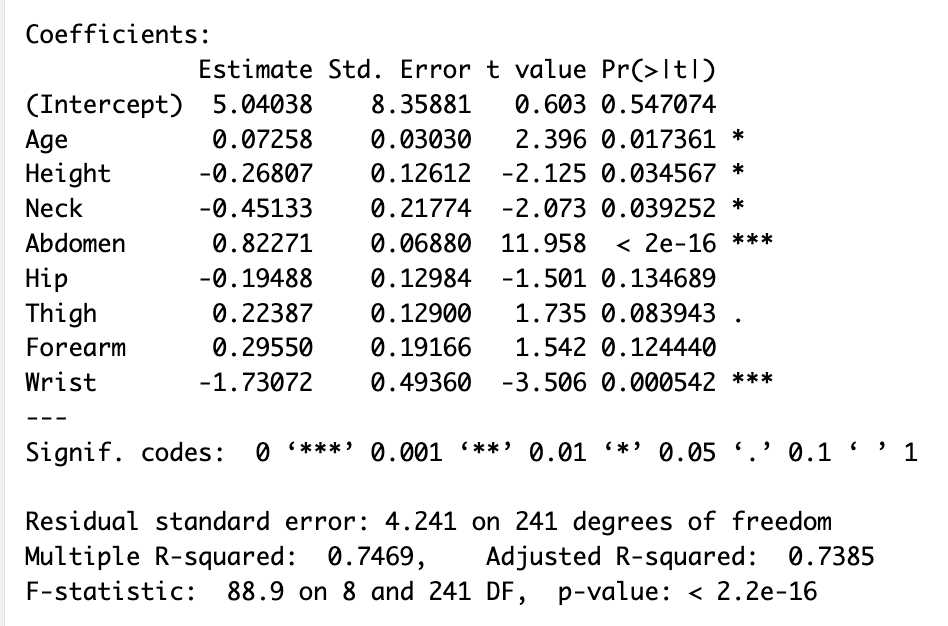
\includegraphics[width=0.9\linewidth]{StepwiseSelection.png}
    \caption{Stepwise Selection Results showing significant predictors.}
    \label{fig:stepwise}
\end{figure}

Using a 5\% significance threshold, we selected Age, Height, Neck, Abdomen, and Wrist as the independent variables for the model.

\subsection*{Fitting the Model}
The Multiple Linear Regression model constructed with these variables is shown in Fig. \ref{fig:linear_model}.

\begin{figure}[!htbp]
    \centering
    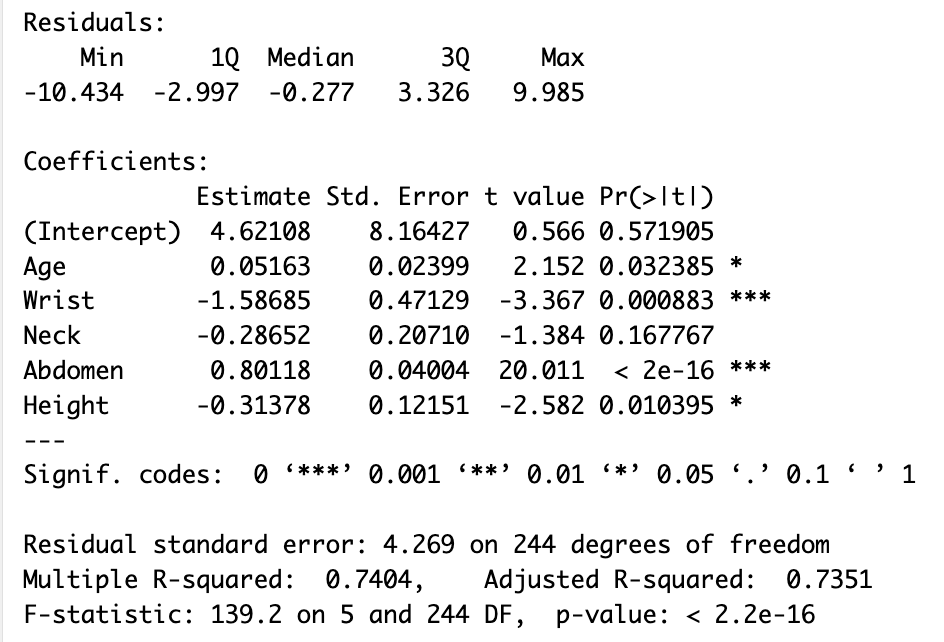
\includegraphics[width=0.9\linewidth]{linear_model.png}
    \caption{Multiple Linear Regression Model for predicting body fat percentage.}
    \label{fig:linear_model}
\end{figure}

\section*{Assumption Checking}
To ensure the validity of our model, we checked key assumptions.

\begin{figure}[!htbp]
    \centering
    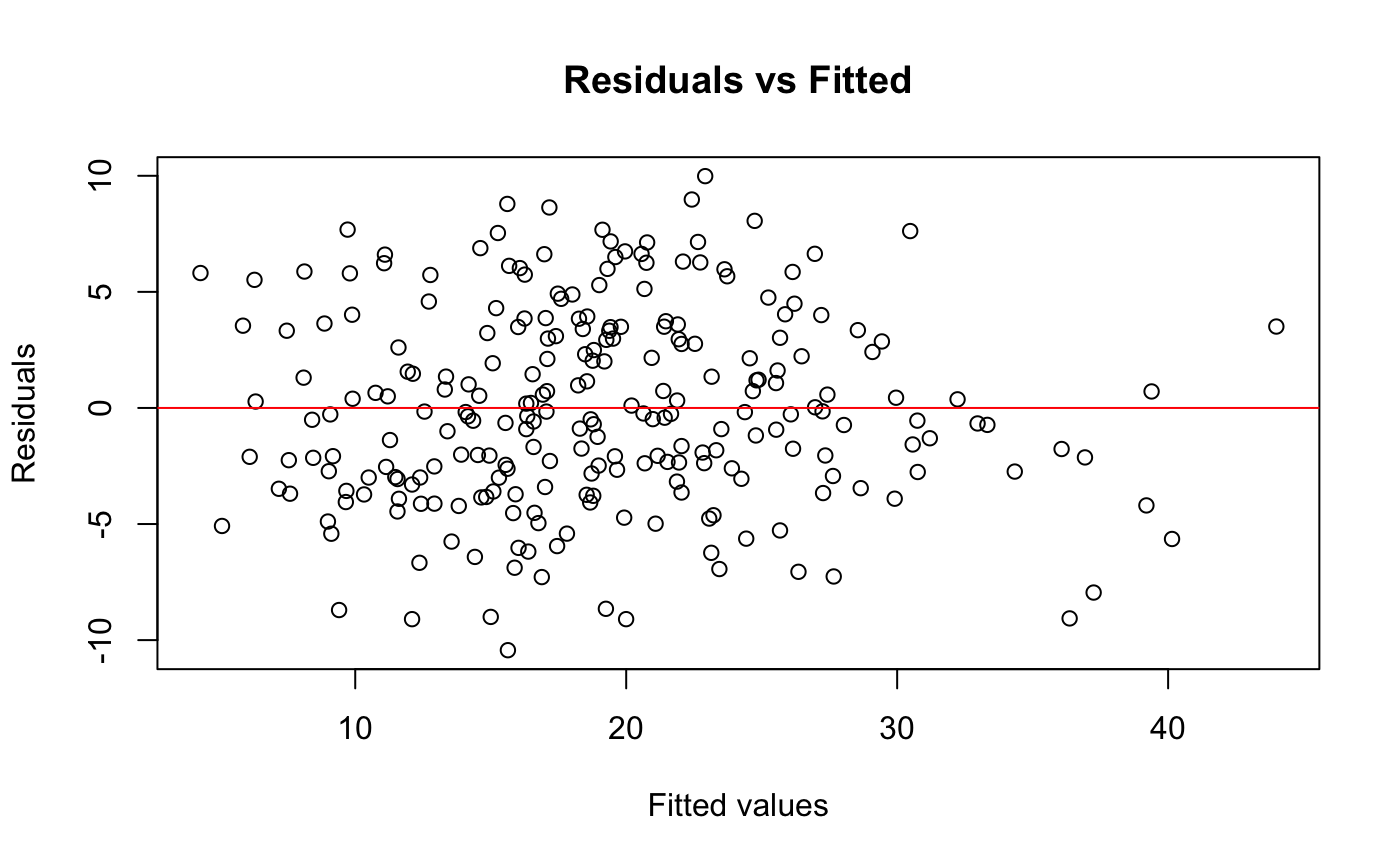
\includegraphics[width=0.7\linewidth]{ResidualPlot.png} 
    \caption{Residual Plot showing residuals scattered around zero, indicating linearity.}
    \label{fig:Residual_plot}
\end{figure}

\subsubsection*{Linearity}
As shown in Fig. \ref{fig:Residual_plot}, the residuals are randomly scattered around zero, indicating the linearity assumption is met.

\subsubsection*{Homoscedasticity}
As shown in Fig. \ref{fig:Residual_plot}, the residuals plot does not show any discernible pattern, confirming that homoscedasticity is maintained.

\subsubsection*{Normality}
The points in the Q-Q plot (Fig. \ref{fig:QQplot}) fall approximately along the line, indicating normality.
\begin{figure}[!htbp]
    \centering
    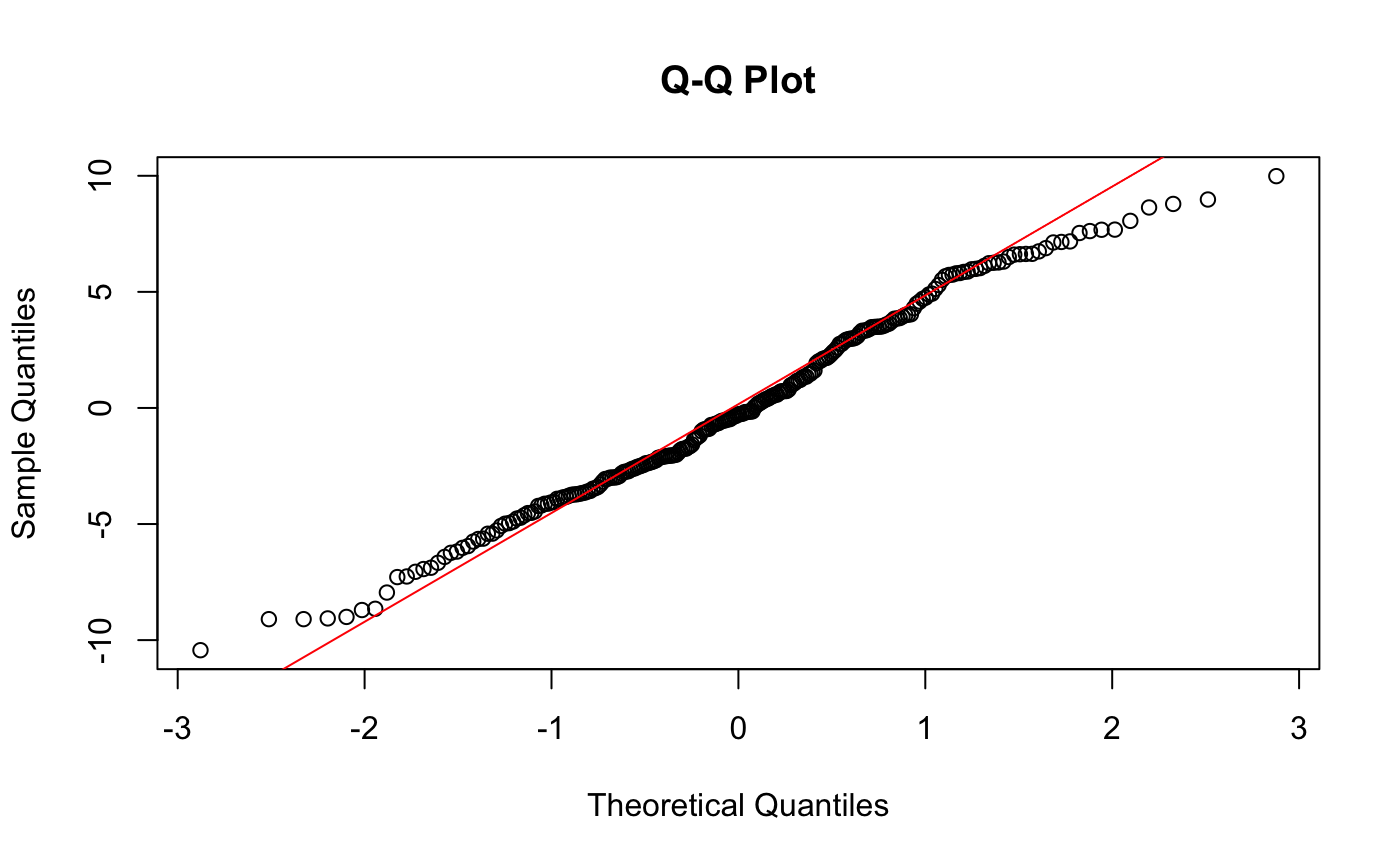
\includegraphics[width=0.6\linewidth]{QQPlot.png} 
    \caption{Q-Q Plot confirming normality assumption.}
    \label{fig:QQplot}
\end{figure}

\subsubsection*{Multicollinearity}
As shown in Fig. \ref{fig:VIF}, all VIF values are less than 5, confirming minimal multicollinearity.
\begin{figure}[!htbp]
    \centering
    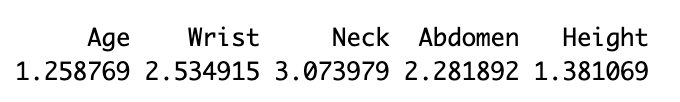
\includegraphics[width=0.6\linewidth]{autocorrelation.png}
    \caption{Variance Inflation Factor (VIF) results indicating multicollinearity levels.}
    \label{fig:VIF}
\end{figure}

\section*{Model Refinement}
We refined the model by identifying and removing influential outliers using Cook’s Distance.

\subsubsection*{Outlier Identification}
Cook's Distance plot (Fig. \ref{fig:Cooks_Distance}) identifies points above the threshold as influential, which were removed for model refinement.
\begin{figure}[!htbp]
    \centering
    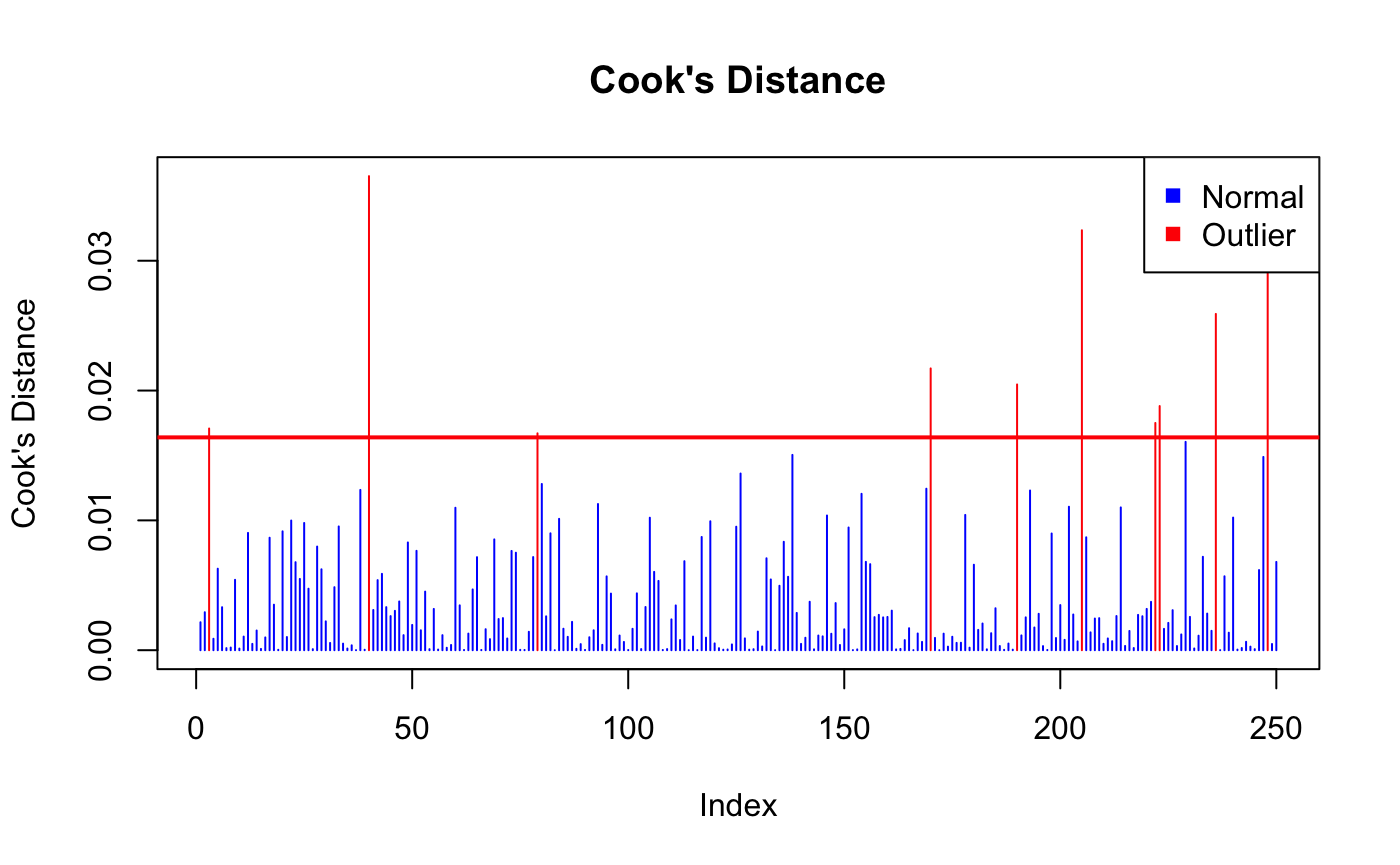
\includegraphics[width=0.8\linewidth]{Cooks_Distance_Image.png}
    \caption{Cook's Distance Plot showing influential data points.}
    \label{fig:Cooks_Distance}
\end{figure}

\subsubsection*{Refined Model}
The refined model (Fig. \ref{fig:Final_Model}) achieved higher accuracy with improved R-squared and lower residual error.
\begin{figure}[!htbp]
    \centering
    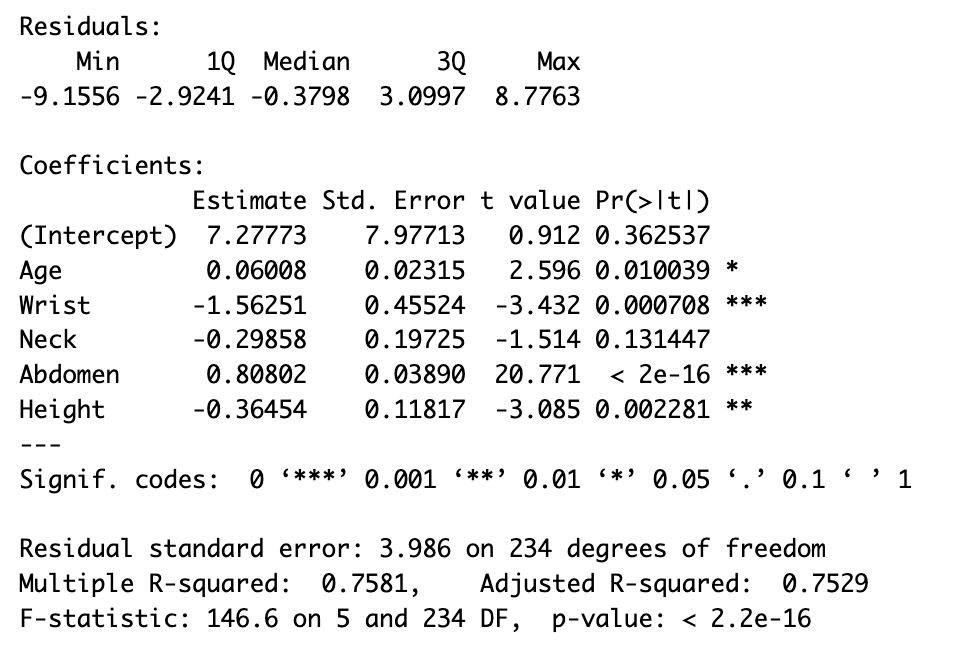
\includegraphics[width=0.9\linewidth]{Final_Model.png}
    \caption{Final refined model with improved R-squared and lower Residual Standard Error.}
    \label{fig:Final_Model}
\end{figure}
\newpage
\section*{Results}

The final predictive model identified \textbf{Age, Height, Neck, Abdomen, and Wrist} as the most significant predictors of body fat percentage, with \textbf{Abdomen} showing the highest correlation. This suggests that abdominal measurements have a strong influence on body fat prediction, which is consistent with known associations between abdominal fat and overall body fat.

After refining the model by removing influential outliers identified through \textit{Cook's Distance}, the accuracy of predictions improved notably. The refined model demonstrated an \textbf{increased R-squared value} and a \textbf{decrease in Residual Standard Error}, indicating a better fit and reduced variance in prediction errors.

\subsection*{Model Performance}

The refined model's performance was evaluated based on metrics like \textbf{R-squared} and \textbf{Residual Standard Error}:
\begin{itemize}
    \item \textbf{R-squared}: The model achieved a high R-squared value which is 0.76, signifying that a large proportion of the variance in body fat percentage could be explained by the selected predictors.
    \item \textbf{Residual Standard Error}: The lower Residual Standard Error in the refined model signifies improved precision in the predictions.
\end{itemize}

\subsection*{Predictor Significance and Interpretation}

\begin{itemize}
    \item \textbf{Abdomen}: As the most influential variable, it highlights a direct relationship with body fat percentage, aligning with findings in health research.
    \item \textbf{Other Predictors} (Age, Height, Neck, and Wrist): These variables, while not as impactful as Abdomen, contribute to refining the body fat estimation, providing a balanced prediction model that does not rely on a single measurement.
\end{itemize}
\section*{Discussion and Conclusion}
In the current study, the sample size of the dataset we used was extremely limited and only male, so the current model is likely to be biased from widespread use. Therefore, in the future, we will collect more data to build and train models to improve their universality.

\end{document}
